\documentclass[a4paper, 12pt]{report}

% Page Margins
\usepackage[a4paper, total={15cm, 24.7cm}]{geometry}
% Charset
\usepackage[utf8]{inputenc}
% Language
\usepackage[british]{babel}
% Font
\usepackage[default]{sourcesanspro}
\usepackage[T1]{fontenc}
\usepackage{titlesec, color}
\definecolor{gray75}{gray}{0.75}
\newcommand{\hsp}{\hspace{20pt}}
\usepackage{microtype}
\usepackage{float}
\usepackage{tabto}
% Color
\usepackage{xcolor}
% Graphics
\usepackage{graphicx}
\usepackage{fancyhdr}
\graphicspath{ {./img/} }
% Indexing
\usepackage{index}
\makeindex
% Hyperlinks
\usepackage{hyperref}
\hypersetup{
 	colorlinks=true, 
	linkcolor=black,
	urlcolor=blue,
	citecolor = black,
}
% Bibliography
\usepackage{comment}
\usepackage[
	backend=biber,
	sorting=ynt
]{biblatex}
\addbibresource{references.bib}

\begin{document}

% Title page
\title{\LARGE{The Bitcoin Lightning Network: A Solution to Bitcoin's Scalability Problem}}
\author{Yannick Mawuena Rüfenacht \\ \href{mailto:yannick.ruefenacht@hotmail.com}{yannick.ruefenacht@hotmail.com}}
\date{October 21, 2020\\Version 1.0.0}
\maketitle

% Quote
\begin{quote}
\vspace*{\fill}
\textit{``The Bitcoin lightning network is a payment protocol designed to allow instant and fee-less Bitcoin payments between two parties. The lightning network works by creating direct payment channels between persons."}
\par\raggedleft--- \textup{CryptoDefinitions}
\vspace*{\fill}
\end{quote}

% Abstract
\begin{abstract}
Today’s Bitcoin protocol provides the opportunity to participate in a secure decentralized payment system that operates on a network of peer-to-peer online transactions without a single bank being in charge of all user accounts. Instead, the users themselves each maintain a copy of all accounts. In order to ensure that each member of the network has the same copy of all accounts, Bitcoin uses the blockchain technology. However, the process of securing and distributing transactions through the blockchain takes up a substantial amount of time, which creates a significant drag on the ability to encompass all global financial transactions. The idea of the lightning network is to create micropayment channels between participants that operate off-blockchain. These channels can be used to instantly exchange Bitcoins without having to distribute them through the blockchain. Upon closing a micropayment channel, the final balance of that channel is broadcasted to the main blockchain. This concept could prove to be useful especially in situations where two participants frequently exchange money.
\end{abstract}

% Table of Contents
\tableofcontents
\listoffigures

% Formatting
\setlength{\parskip}{1em}
\setlength{\parindent}{0em}
\titleformat{\chapter}[hang]{\LARGE\bfseries}{\thechapter\hsp\textcolor{gray75}{|}\hsp}{0pt}{\LARGE\bfseries}
\titleformat{\section}[hang]{\large\bfseries}{\thesection\hsp\textcolor{gray75}{|}\hsp}{0pt}{\large\bfseries}

% Page bottom transition
%\widowpenalties 1 10000
%\raggedbottom

\chapter{Introduction}

\par The primary aim of this paper is to provide a simple to understand explanation of the Lightning Network and why it is necessary. Furthermore, this paper also dives into the underlying system upon which the Lightning Network operates, namely the Bitcoin blockchain system. The Lightning Network uses the blockchain to create a secure network of participants which are able to perform transactions at high volume and speed. To be able to understand how the lightning network works or why it is even necessary, requires a basic understanding of the blockchain and Bitcoin.

\par This paper guides the reader through a list of steps that show how the lightning network works, starting from the basics of a decentralized payment protocol. Each step builds on top of the previous one. It is therefore recommended to read this paper in the right order.

\chapter{A Brief Overview of the Bitcoin Blockchain}

\par In the past there have been many attempts to create a perfectly decentralized payment system. However, the idea of implementing such a payment system had been proven to be quite difficult. There were many problems and loopholes that came to the surface and had to be fixed. With each iteration of a new protocol, a new problem was fixed, and the security had increased. Today’s Bitcoin protocol is the result of all the steps that needed to be implemented to create a secure decentralized payment system.

\section{The Problem with Ordinary Banking Systems}

\par The way of ordinary banking systems usually goes as follows: When Alice wants to transmit one coin to Bob, she sends her transaction to a central bank, where all the balances of all the customers are stored in a database, or ledger. The bank then proceeds to process Alice’s transaction by updating the values of Alice and Bob accordingly, which concludes the transaction. 

\begin{figure}[H]
	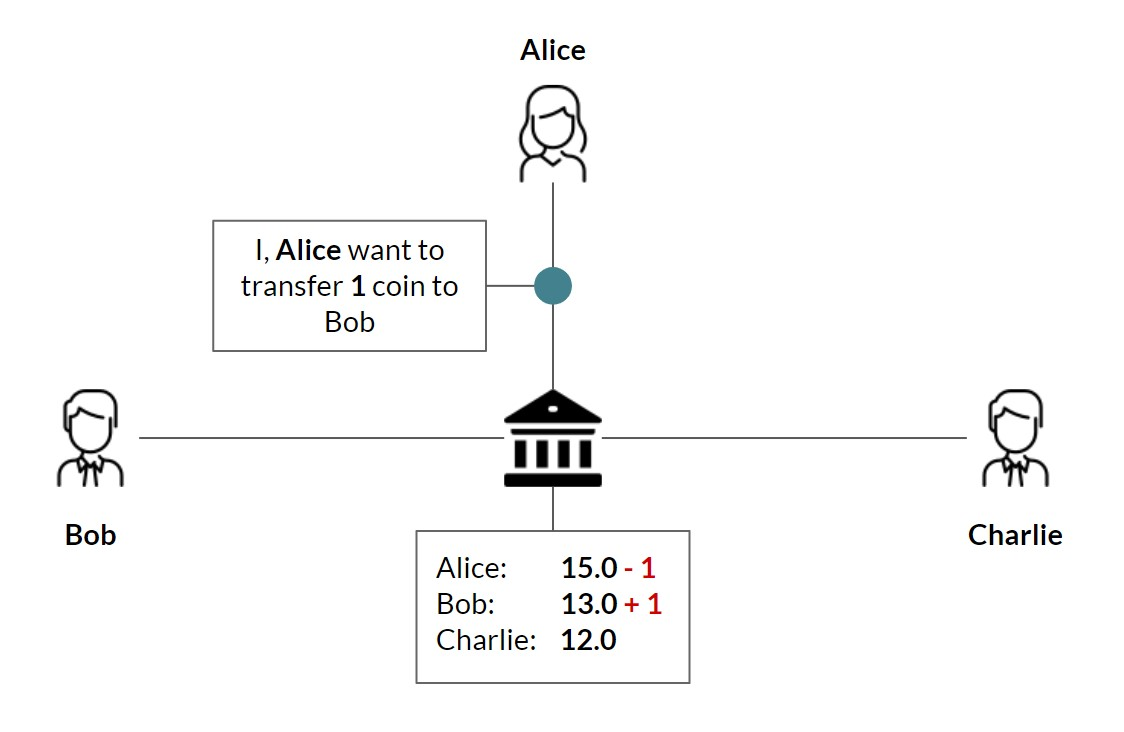
\includegraphics[width=\textwidth]{01_Banking_System}
	\caption{Traditional Banking System}
	\medskip
	\small \textit{In a traditional banking system, the bank is in full control of handling transactions and managing balances, which gives it a lot of power.}
	\label{fig:01_Banking_System}
\end{figure}

\par The underlying concern in this system is that one entity, namely the bank, is in full control of the balances of all the users. That said, the bank has the capability to:

\begin{itemize}
	\item \textbf{Generate money at will.}\\The bank could for example change the balance of Alice from 14.0 to 20.0, which generates 6.0 extra coins.
	\item \textbf{Steal money at will.}\\Or if the bank decides to shorten Alice’s balance from 14.0 to 10.0, then 4.0 coins will be stolen.
	\item \textbf{Censor transactions.}\\Since the bank is the receiver of all the transactions, it has the power to simply ignore incoming transactions, thereby censoring them.
\end{itemize}

\par The inner workings of the bank are strictly sealed to the outside world, which has the potential to create trust issues. And this is where the idea of Bitcoin comes into play.

\section{The Idea of Decentralization}

\par The main idea of Bitcoin is to remove the central entity that is in control of the ledger containing all balances, and to form a network of users where everyone is connected to everyone and the same rights apply to everyone.

\par To achieve this kind of system, the ledger would not be stored in one central place anymore, but instead, every participant of the network obtains their own copy of the ledger and updates it accordingly. That way each participant fulfils the role of a bank on their own.

\par If Alice now wants to transfer one coin to Bob, she no longer sends her transaction to the bank, but instead, she updates her own ledger first and then sends it to the other participants on the network, so that they can update their ledgers as well.

\begin{figure}[h]
	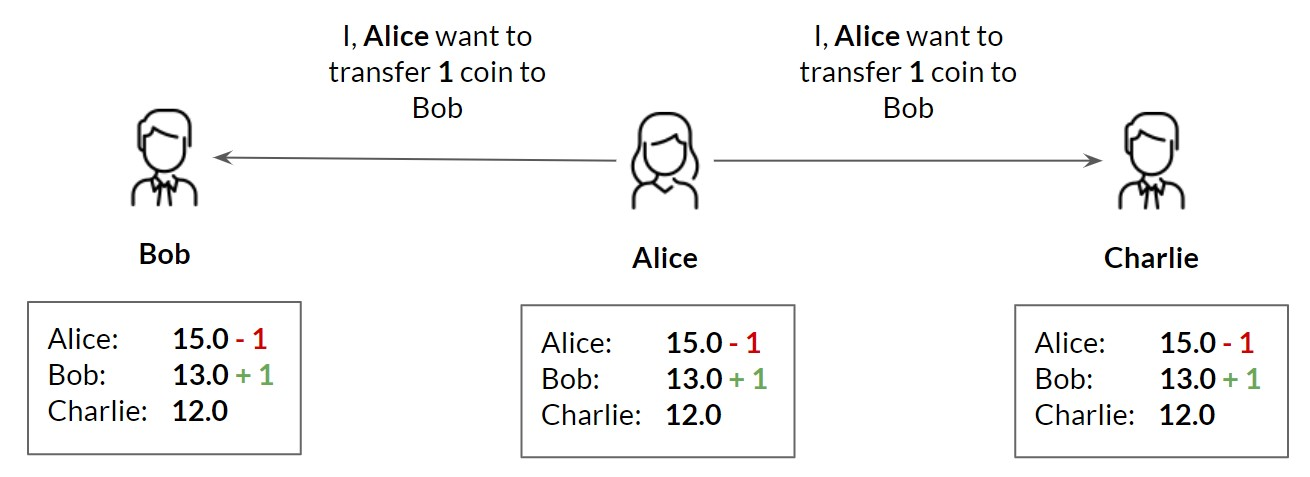
\includegraphics[width=\textwidth]{02_Naive_System}
	\caption{Decentralized Payment System}
	\medskip
	\small \textit{In a decentralized system, the bank is removed and everyone keeps track of all the balances by themselves. When someone performs a payment, they now need to inform all the other users in the network.}
	\label{fig:02_Naive_System}
\end{figure}

\par At first, the degree of openness that this system provides might seem absurd. But the fact that all the records of the transactions are publicly available also means that everyone can verify the validity of every transaction. And this is where a decentralized system gains its immense trust and security benefits.

\section{The Issue of Decentralization}

\par Although the idea of removing an all-powerful centralized entity seems quite appealing so far, the actual implementation of a decentralized system is far more complex. In Bitcoin, there are several security mechanisms involved that aim to establish a stable network without coin theft. The main concern of a decentralized system, where all transactions are publicly distributed to every node of the network, is to ensure that every node has the same history of transactions. In the Bitcoin network, each transaction has a reference to its previous transaction, similarly to a linked list, which establishes a fixed order of transactions.

\par Nonetheless, this alone cannot guarantee the right order of transactions for every participant. From a performance perspective, the idea of everyone publicly broadcasting their transactions to the entire network would work for a small number of people, however, as the number of participants increases, it becomes significantly more difficult to maintain the right order of transactions across the entire network. Network delays could cause transactions to arrive in different orders in different places.

\par To see why it is important that the ledger, the history of all transactions, has the same order of transactions across the entire network, becomes very apparent when looking at the Double Spending Problem.

\section{The Double Spending Problem}

\par The Double Spending Problem describes a scenario, where one party uses the same money to pay two different parties at once. In the real world, this would not be possible. If a coin is spent once, it is physically gone. However, in a digital payment system, a coin is just a digital value that can be copied very easily, as demonstrated in the following scenario:

\par Alice has a total balance of 1 mBTC. She uses that money to pay Bob in exchange for one of his books. By doing so, a new transaction (T1495) is created and added to the ledger. This transaction contains a reference to its previous transaction (T1494). After Bob receives the money, he proceeds to send Alice his book, and the payment is complete. After a while, Alice discovers a shirt in Charlie’s shop that she really likes, which costs 1 mBTC, just as the book. Alice, who has no money left at this point, decides to cheat the system by creating a new transaction that points to transaction 1494 as its previous one, making it seem as if this is the 1495th transaction, when in fact it is actually the 1496th one. From Charlie’s perspective this seems like a valid transaction, so he accepts it. With that, Alice has used 1 mBTC to pay for two items that each cost 1 mBTC.

\begin{figure}[h]
	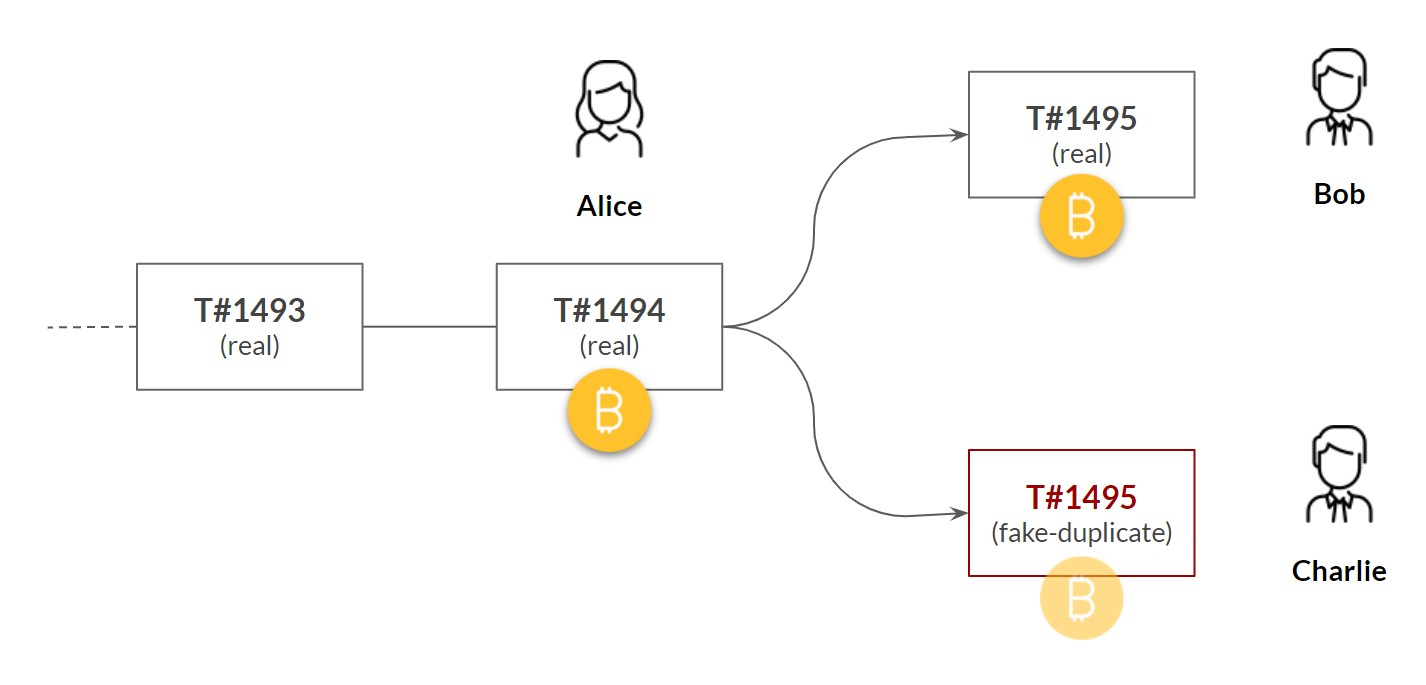
\includegraphics[width=\textwidth]{03_Double_Spend}
	\caption{The Double Spending Attack}
	\medskip
	\small \textit{After paying Bob with transaction no. 1495, Alice goes back in time in the blockchain to transaction no. 1494 where she still had 1 coin left, and creates a new transaction from that point in time to pay Charlie.}
	\label{fig:03_Double_Spend}
\end{figure}

\section{The Computational Puzzle}\label{chap:The_Computational_Puzzle}

\par The Double Spending Problem was first solved in 2008 by Satoshi Nakamoto. The way he solved the problem is by adding a computational puzzle that needs to be solved before a transaction can be published and broadcasted into the network. A computational puzzle is a problem that is hard to solve but easy to verify. This puzzle is set up in a way, that it needs a lot of computing power to be solved, which establishes two main rules:

\begin{itemize}
	\item The generation of new transactions is now proportional to the computing power required to solve the puzzle. This makes it extremely difficult for an organisation to overtake the network, as it now needs the corresponding computing power and not merely the majority of nodes in the network.
	\item The creation of transaction is now regulated. Not anyone can now simply create a new transaction, instead, a leader is chosen. The person who solves the puzzle becomes leader and has the right to publicly announce and broadcast the transaction. Incoming transactions are now only valid if they stem from the leader.
\end{itemize}

\par The addition of a computational puzzle does not mean that every user now needs to solve a puzzle before they can publish a transaction. In practice, when a transaction is created, it is sent to a waiting pool. From there, special members of the network known as “Minors” will solve the puzzles and broadcast the transactions. It takes on average 10 minutes to complete one puzzle. To compensate the minors for the work that they contribute to secure the network, they are rewarded with small amounts of Bitcoin that become available to the miner when the puzzle is solved.

\section{The Bitcoin Blockchain}

\par The implementation of a computational puzzle for each broadcast has greatly increased the stability of the network as the generation of new transactions is now regulated. However, there is still a chance that two minors solve thier puzzles at the same time so that two different transactions are being broadcasted simultaneously, which is also known as a “Soft Fork”. This results in different parts of the network having a different order of transactions.

\par This problem is solved with the implementation of the blockchain. In the blockchain, transactions are grouped into blocks, where each block has its puzzle and a reference to its previous block. This chains all the blocks together, hence the name: blockchain.

\begin{figure}[H]
	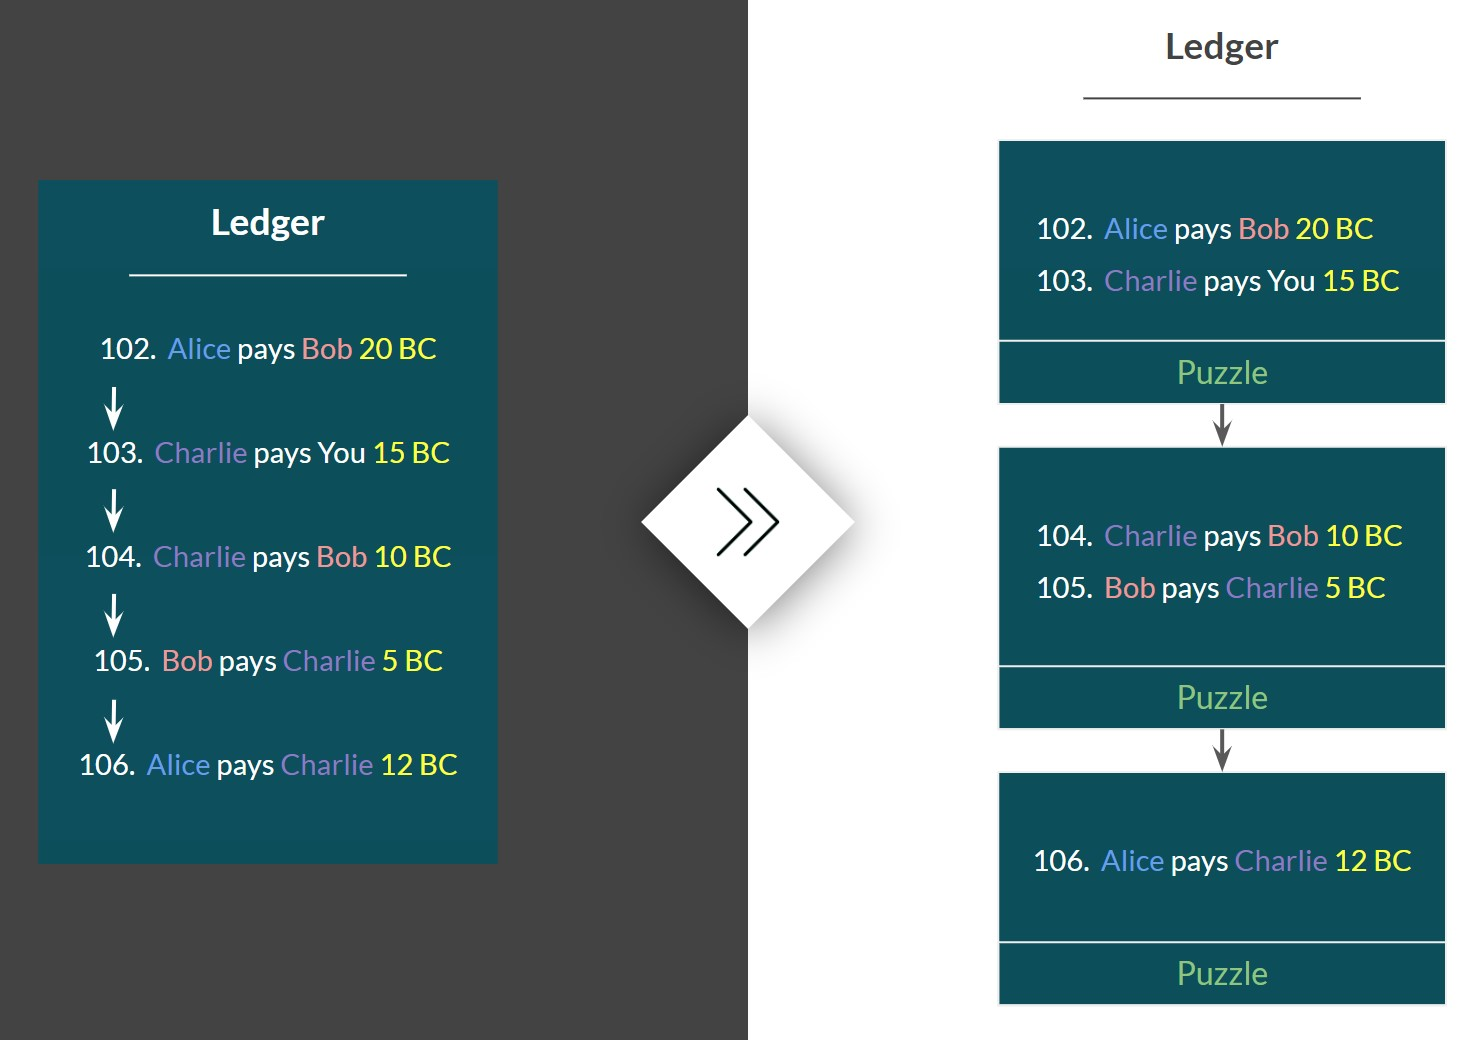
\includegraphics[width=\textwidth]{04_Ledger_Split}
	\caption{Ledger is split into blocks}
	\medskip
	\small \textit{Instead of distributing one file that contains the history of transactions, it is much more efficient to distribute the list as separate chunks of data accross the Bitcoin network.}
	\label{fig:04_Ledger_Split}
\end{figure}

\par Now, if one receives two blocks that point to the same previous block, one must simply follow the chain, which is the longest, since it has the most computational work put into it. Generally, a block can be considered confirmed after a few more blocks have arrived on the chain. This is the reason why Bitcoin has long confirmation times.\cite{grant}

\begin{figure}[H]
	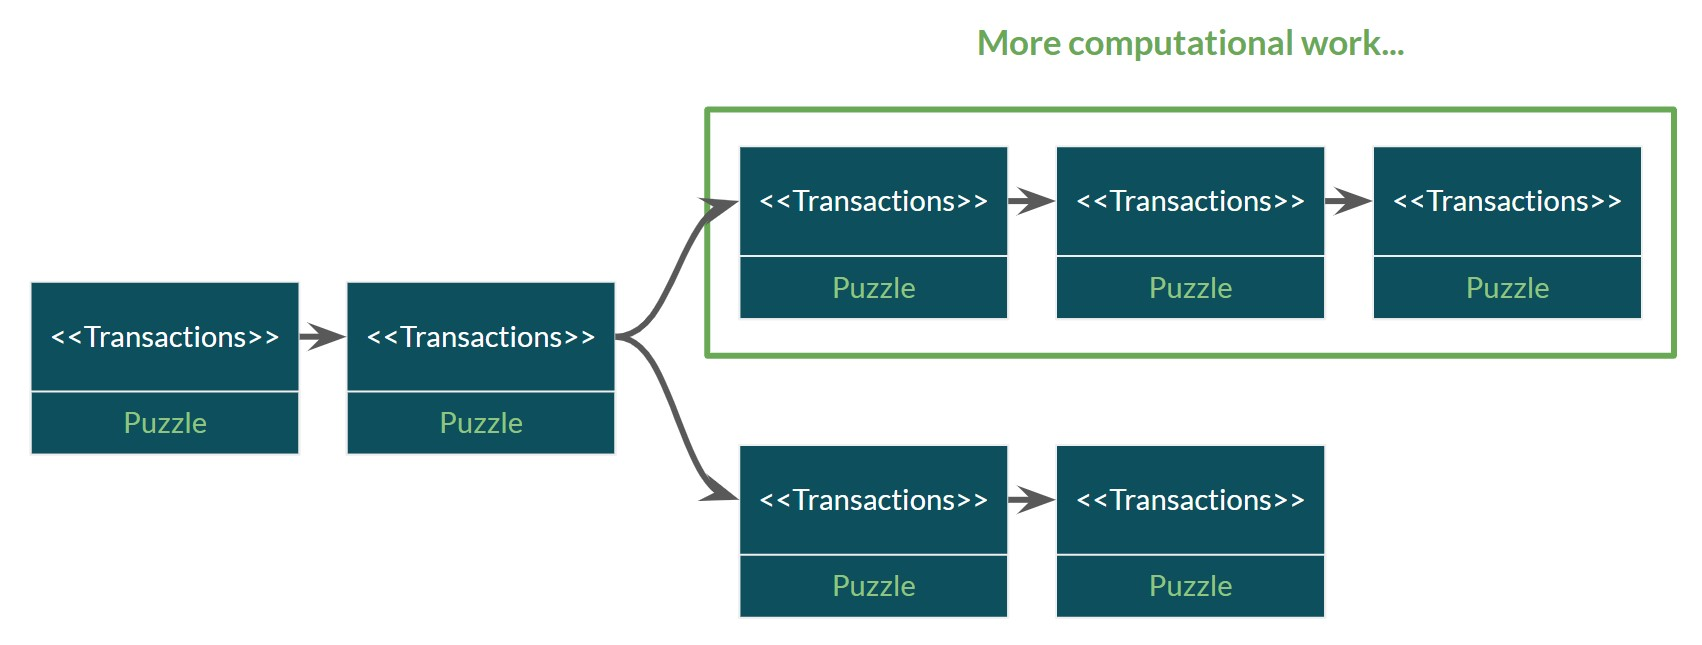
\includegraphics[width=\textwidth]{05_Soft_Fork}
	\caption{Soft fork}
	\medskip
	\small \textit{In the event of two blocks being broadcasted simultaneously, there will be two parts of the network with conflicting transaction histories, which results in a fork in the blockchain. In that case, users must simply follow the chain which is the longest, since it has the most computational effort put into it.}
	\label{fig:05_Soft_Fork}
\end{figure}

\chapter{The Scalability Problem with Bitcoin}

\par The Bitcoin scalability problem is the limited rate at which bitcoin transactions can be processed. This problem ties in with the fact that blocks have a limited size and can only be generated once every 10 minutes, due to the computational puzzle. Also, considering that each block needs to be broadcasted worldwide to all the nodes of the network, that intend to update the blockchain, might create significant time delays for some users. For these reasons, Bitcoin by itself is only able to handle a few transactions per second and will thus not be able to handle the whole transaction volume of the world anytime in the near future.\cite{joseph}

\section{Bitcoin Blockchain Fees}

\par As explained in chapter~\ref{chap:The_Computational_Puzzle}, minors are the ones who add blocks to the blockchain by solving the computational puzzle. For that work, miners are to be rewarded with small portions of Bitcoin, that are stored in each block. However, users may also provide additional amounts of Bitcoin to a transaction to incentivise the minors to process their transaction earlier than others. If the demand for Bitcoin rises, i.e., more transactions are generated, higher bids will be placed on transactions, the same way the other way around. This causes fee instability, which is a problem for those users who are accustomed to place low bids and cannot afford to pay high bids. This inconsistency of fees could prevent Bitcoin from scaling to a large user base, that uses Bitcoin regularly.\cite{daniel}

\chapter{Introducing the Lightning Network}

\par The Lightning network presents an additional layer that operates on top of the Bitcoin blockchain with the aim to enable instant and feeless micropayments. It has been introduced in late 2015, early 2016, and has been in development ever since. The main idea of the Lightning Network is to establish separate peer-to-peer connections between participants to enable fast transactions. As discussed earlier, the Bitcoin blockchain strongly regulates the creation of new transactions. Additionally, each transaction has a high fee and long confirmation time, which makes it impractical to use Bitcoin for small and quick payments. For that reason, the Lightning Network aims to not store every transaction on the main blockchain, but rather off-blockchain, where they do not need to undergo a long and complicated confirmation process. These connections that are formed between nodes of the Lightning Network are named micropayment channels, or simply payment channels.

\section{Payment channels}

\par If two participants regularly exchange Bitcoin, they would open a new payment channel between them, that is off-blockchain. This allows them to perform quick payments between each other. Once they conclude their business, they conduct a closing transaction which contains the final balances of their wallets from the payment channel. Only the initial and closing transaction are stored on the main blockchain. That way, even if thousands of transactions are performed on the payment channel, only two transactions will be stored on the blockchain eventually.

\paragraph{Creating a new payment channel} \hspace{0pt} \\
During the initiation of the payment channel, both parties provide a certain balance of Bitcoin onto their ends of the payment channel, allowing that balance to go back and forth between them whenever transactions are made. To complete the creation of the new payment channel, the inputs of both parties are put into a transaction that gets signed by both parties, and eventually, broadcasted on the main blockchain. This transaction is called the funding transaction.

\paragraph{Commitment transactions} \hspace{0pt} \\
Once the funding transaction has been added to the blockchain and settled, both parties can spend their balances on the channel in a series of commitment transactions that reallocate their balances accordingly. These kinds of transactions remain between the channel participants and do not need to be stored on the blockchain.

\paragraph{Closing the payment channel} \hspace{0pt} \\
The balances of both parties can remain off-blockchain and be updated continuously until finally a settlement transaction is performed. This transaction contains the final balances of both parties and gets added to the main blockchain.

\paragraph{Examples} \hspace{0pt} \\
In this example money flows both ways in the payment channel, therefore it is considered a bi-directional payment channel.\cite{andreas}

\begin{figure}[H]
	\centering
	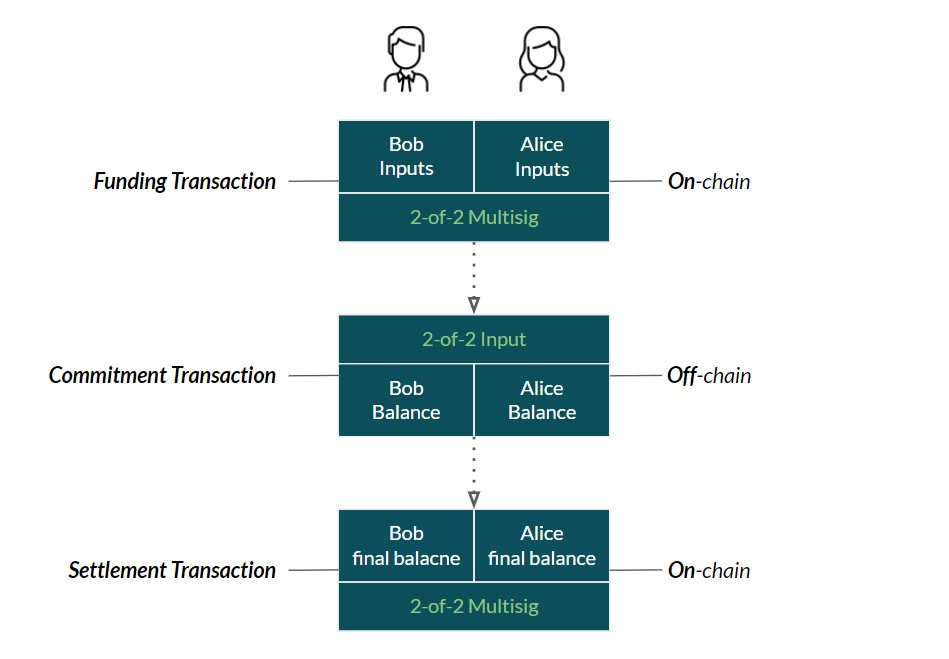
\includegraphics[width=13cm]{06_Bidirectional_Channel}
	\caption{Bi-directional payment channel}
	\medskip
	\small \textit{In a bi-directional payment channel both parties have their own balance which they can use to exchange coins. Since money flows in both directions, it is considered a bi-directional payment channel.}
	\label{fig:06_Bidirectional_Channel}
\end{figure}

\par Naturally, there can also be payment channels where money only flows in one direction, from one party to another. The example below demonstrates how a payment channel could be used to perform micropayments to an internet service provider in exchange for mobile data.

\begin{figure}[H]
	\centering
	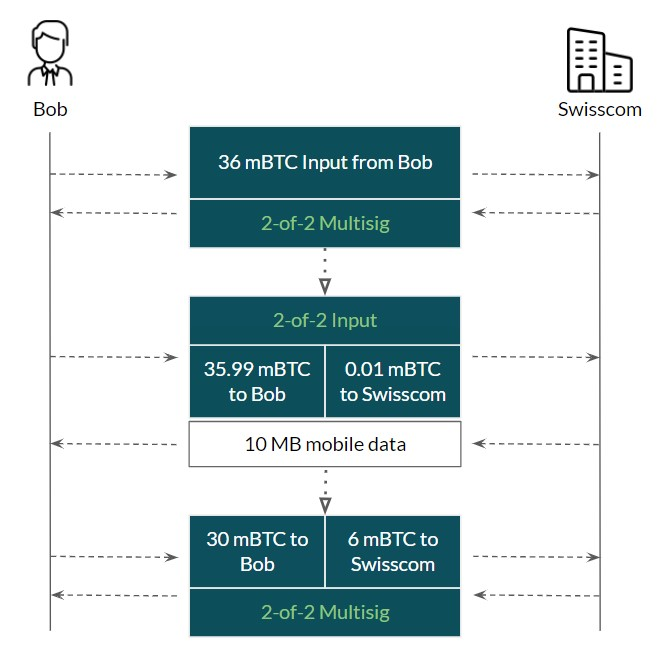
\includegraphics[width=10cm]{07_Onedirectional_Channel}
	\caption{Example of a payment channel to pay for mobile data usage}
	\medskip
	\small \textit{This example shows how payment channel could be used to pay miniscule amounts of Bitcoin in exchange for small chunks of data.}
	\label{fig:07_Onedirectional_Channel}
\end{figure}

\paragraph{Security} \hspace{0pt} \\
Payment channels rely on Bitcoin security primitives which prevent participants from stealing Bitcoin or losing Bitcoin due to uncooperative behaviour from the opposite party. Such security primitives include Multi-Signatures, Timelocks and No-Double-Spends.

\section{Multi-Signatures}

\par As the name suggests, the idea behind Multi-Signature technology is to have multiple signatures or keys be in control of a Bitcoin balance. Multi-Signatures are described as “K of N” signature schemes, meaning that there are N valid predefined signatories that are authorized to release funds from a particular Bitcoin balance. Of those N keys, K is the number of signatures that are required to sign a transaction.\cite{inbook}

\paragraph{2 of 2 Multi-Signature} \hspace{0pt} \\
In the case of the Lightning Network, a “2 of 2 Multi-Signature” type is used. This requires both parties of the channel to sign any transaction, because of that, one party alone cannot sign and execute a transaction on their own.

\section{Timelocks}

\par A payment channel gets closed when either party decides to publish the latest transaction onto the blockchain. That said, there is one major security concern to be found here. If, for example, Bob and Alice are using a payment channel in which, according to the latest commitment transaction, Alice has a greater Balance than Bob, the Question arises: Can Bob not simply broadcast a prior state in which he had a more advantageous balance and thus cheat?

\par The way this can be solved is to set a “timelock”. A timelock is an embedded delay or countdown in a commitment transaction that determines when the transaction becomes valid. Later commitment transactions have a shorter timelock and will therefore become valid sooner. This prevents either party from spending an older commitment transaction.

\begin{figure}[h]
	\centering
	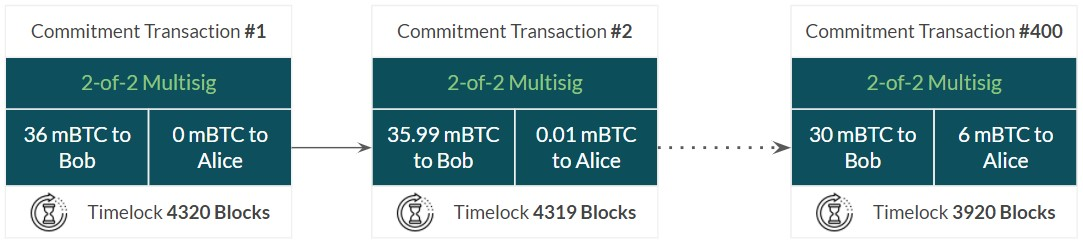
\includegraphics[width=13cm]{08_Timelocks}
	\caption{Timelocks}
	\medskip
	\small \textit{Transaction number 400 has the smallest timelock and thus becomes valid sooner than every other transaction.}
	\label{fig:08_Timelocks}
\end{figure}

\section{No Double-Spend}

\par Once a commitment transaction has been broadcasted and its timelock has finished, it becomes a legitimate transaction and all the other commitment transactions automatically become invalid, since there can only be one final settlement transaction per payment channel. This prevents the act of Double Spending a coin. As seen in the picture \ref{fig:08_Timelocks}, transaction number 400 is the first one to become valid and once it does, the other 399 transactions become invalid, which makes it impossible for Bob to cheat and spend the first transaction, where he had 36 mBTC instead of 30mBTC.

\section{Routing}

\par Another way to look at payment channels is to picture them as strings of beads stretched between two people. If Alice has to pay Bob, she can simply push one of her beads to his side. If Bob also has a payment channel with Charlie, Alice can pay Charlie through Bob, meaning that she pushes one of her beads to Bob first, and then Bob pushes one of his beads over to Charlie.

\begin{figure}[H]
	\centering
	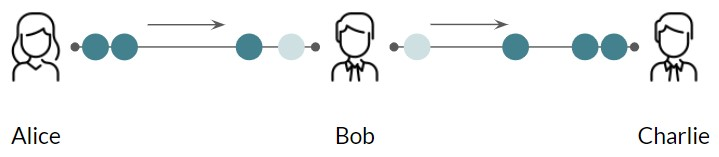
\includegraphics[width=12cm]{09_Beads}
	\caption{Routed payment}
	\medskip
	\small \textit{Alice can pay Charlie through Bob by paying Bob first and then letting Bob pay Charlie.}
	\label{fig:09_Beads}
\end{figure}

\par The idea of people being able to forward payments from one person to another, is called routed payments. If the network of the participants is sufficiently enough connected, everyone will be reachable within a certain number of hops from one end to another. That is precisely what the Lightning Network is all about.

\section{Hash and Timelock Contracts}

\par The concept of routed payments is an essential part of the Lightning Network. Therefore, it is all the more important that it provides the appropriate security mechanisms to prevent coin theft.

\par Payment channels use what is known as “locks contracts” to secure transactions. Locks can be placed around beads to constrain their movement. The Lightning Network uses two types of locks: the hash and time lock. The hash lock is a type of lock that only opens when provided with the correct password. The time lock on the other hand opens automatically after a specified time delay.\cite{peter}

\begin{figure}[H]
	\centering
	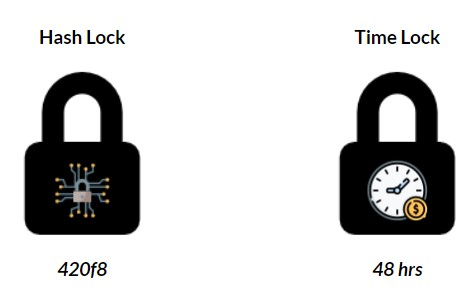
\includegraphics[width=9cm]{10_Locks}
	\caption{Hash and Time lock}
	\medskip
	\small \textit{The hash lock opens when presented with a password that hashes to the specified hash (420f8 in this case). The time lock opens after the specified time has elapsed (48 hours in this case).}
	\label{fig:10_Locks}
\end{figure}

\par If a routed payment is performed, for example, if Alice wants to pay Charlie through Bob, all members need to participate in an elaborate series of steps.

\paragraph{Step 1} \hspace{0pt} \\
First, Charlie thinks up a secret password and tells Alice the password’s hash. In this example the password is “Balderdash”, and its hash is “420f8”. In the next step, Alice uses that hash to send a password protected bead over to Bob. She does this by placing a hash lock around the bead that opens only when presented with a password that hashes to “420f8”. In addition to that, she also places a time lock around the bead that opens automatically after 48 hours and returns the bead to Alice if Bob does not participate in this transaction procedure.

\begin{figure}[H]
	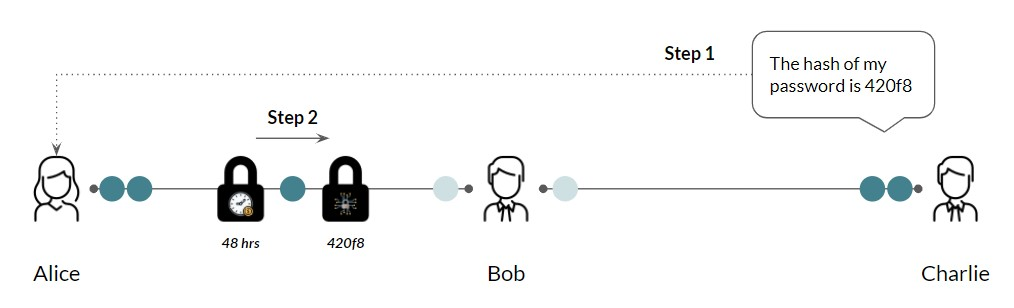
\includegraphics[width=\textwidth]{11_HTLC_Step1}
	\caption{Alice sends bead with hash lock to Bob}
	\medskip
	\small \textit{Charlie thinks up a password and sends Alice the password’s hash. Next, Alice sends a bead over to Bob that is protected with a hash and time lock. Bob can only receive this bead if he knows the password. If Bob does not receive the bead within 48 hours, it is returned to Alice.}
	\label{fig:11_HTLC_Step1}
\end{figure}

\paragraph{Step 2} \hspace{0pt} \\
Bob now knows that he receives the bead if he can figure out the password within 48 hours. He also knows that Charlie will reveal the password to him in exchange for one of his beads. Therefore, Bob places the same hash lock and another time lock around his bead and pushes it over to Charlie. In order for Charlie to open the hash lock, he needs to enter the password in plain in plain sight, which is the same password Bob needs to open the hash lock from Alice.

\begin{figure}[H]
	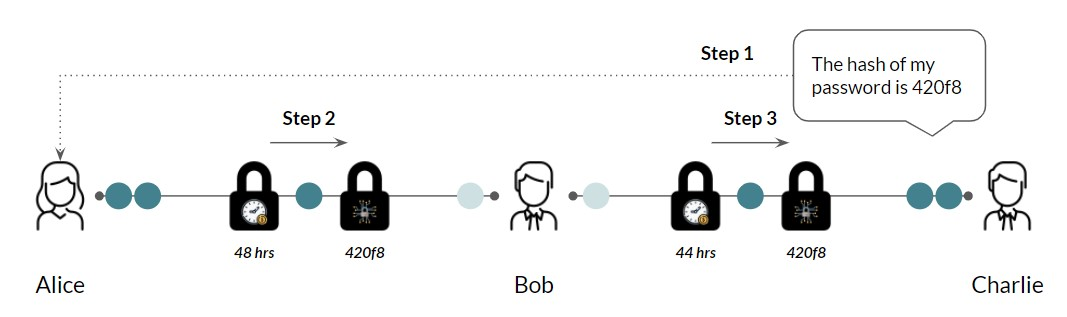
\includegraphics[width=\textwidth]{12_HTLC_Step2}
	\caption{Bob sends bead with copy of Alice's hash lock to Charlie}
	\medskip
	\small \textit{Bob knows that the bead from Alice will be his, if Charlie reveals the password of Alice's hash lock within the 48 hours time frame. He places the same hash lock around one of his beads, adds a time lock, and pushes it to Charlie. The only way Charlie can take the bead is to reveal her password that Bob needs to claim the bead from Alice.}
	\label{fig:12_HTLC_Step2}
\end{figure} 

\paragraph{Step 3} \hspace{0pt} \\
Charlie then enters “Balderdash” into the hash lock and receives the bead from Bob. The lock’s CPU confirms that hash(“Balderdash”) = 420f8, and then opens.

\begin{figure}[H]
	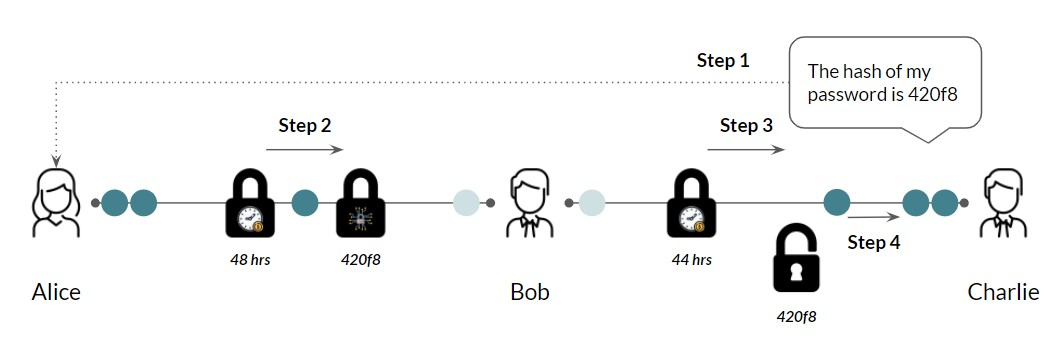
\includegraphics[width=\textwidth]{13_HTLC_Step3}
	\caption{Charlie reveals password and takes his bead}
	\medskip
	\small \textit{Charlie enters his password into Bob's hash lock to open it and take the bead. This reveals the password to Bob.}
	\label{fig:13_HTLC_Step3}
\end{figure} 

\paragraph{Step 4} \hspace{0pt} \\
With knowledge of Charlie’s password, Bob unlocks the hash lock from Alice in the same way and receives his bead. With that, the routed payment is complete.

\begin{figure}[H]
	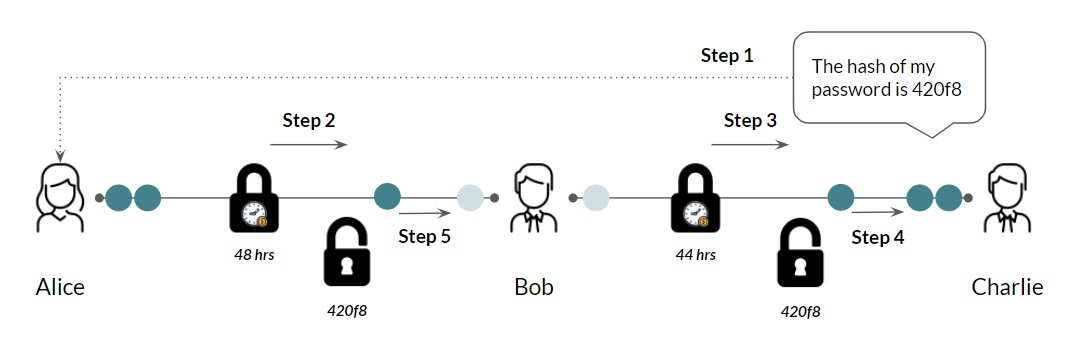
\includegraphics[width=\textwidth]{14_HTLC_Step4}
	\caption{Bob receives his bead from Alice with Charlie's password}
	\medskip
	\small \textit{With knowledge of Charlie's password, Bob can now open the hash lock from Alice and take his bead. This completes the payment.}
	\label{fig:14_HTLC_Step4}
\end{figure} 

\paragraph{Bob’s motivation} \hspace{0pt} \\
When looking at this example, in particular on the role of Bob, one might wonder why Bob would even bother to participate in this whole ritual in the first place if there is nothing in it for him. In practice, however, Alice would add a small additional amount of Bitcoin to her payment for Bob, as a means of motivating Bob to forward the payment and compensating his effort. When the payment is complete, Bob would have slightly more Bitcoin than he started with. The concept of Lightning Network fees will be discussed in more detail in chapter~\ref{sec:Lightning_Network_Fees}.

\paragraph{Uncooperative behaviour} \hspace{0pt} \\
Should a transaction fail, for any reason, as well as uncooperative behaviour, the time lock will enable the affected participants to retrieve their funds. For example, if Bob becomes uncooperative after Alice shifts her bead over, the time lock is what allows Alice to get her bead back. She just needs to wait for the time lock to expire. Since Bob needs the password from Charlie to receive Alice’s bead, which he can only attain by sending one of his beads to Charlie, there is no possibility for Bob to steal Alice’s bead.

\section{Lightning Network Fees} \label{sec:Lightning_Network_Fees}

\par When a participant performs a payment that is routed through several users until it reaches its destination, there needs to be enough capital available on the routes that the payment goes through. If there is not enough liquidity available on the routes, then it becomes impossible to route payments.

\par The Lightning Network is setup in a way that rewards participants who provide liquidity to the network. Should a user choose to route payments, they can set fees that other users will have to pay to use their capital for routing.\newline
There are two types of fees: The \textit{base fee} and the \textit{liquidity provider fee}.\cite{chris}

\paragraph{Base Fee} \hspace{0pt} \\
The base fee is a flat rate that a user charges per transaction that is routed through their node in the network. This fee is set by every user based on what they think their capital is worth. Someone for instance might set their base fee to 0.1 mBTC while someone else, who perhaps is not as liquid, might set their base fee to 0.3 mBTC.

\paragraph{Liquidity Provider Fee} \hspace{0pt} \\
This fee is charged based on how much Bitcoin is routed though one’s payment channel. An example would be a fee of 0.01 mBTC for every mBTC that is routed through one’s payment channel.

\paragraph{Full example} \hspace{0pt} \\
Assuming Charlie needs to pay Alice 5 mBTC through Bob, and Bob has the following Lightning Network Fees: 

\begin{itemize}
	\item[--] Base Fee: \tab \textit{0.1 mBTC} 
	\item[--] Liquidity Provider Fee: \tab \textit{1\% of payment amount} 
\end{itemize}

The fee for Charlie’s lightning payment would result to a total of:\\
Base fee + liquidity provider fee, which equals: 0.1 + (5 * 0.01) = \textbf{0.15 mBTC}

\paragraph{Comparison to traditional Bitcoin blockchain} \hspace{0pt} \\
A traditional node in the Bitcoin blockchain does not generate any money for its owner. All fees collected go directly to the miners. On the Lightning Network however, there are no miners, and all the fees go to the node owners. This key difference also aims to encourage decentralization.

\chapter{Disadvantages of the Lightning Network}

\par The Lightning Network provides very practical benefits for the use of cryptocurrencies. There are, however, a few disadvantages that come with it.

\paragraph{No support for offline payments} \hspace{0pt} \\
Should a user want to send, receive, or forward a payment, they would need to be online at that time. This means that, in order to successfully complete a payment, all affected parties must be online at least once. This can cause an inconvenience to those users who might not always have access to the internet.

\paragraph{Long waiting times for refunds} \hspace{0pt} \\
When a party is uncooperative or unresponsive during a transaction process, the affected party must wait several hours, or potentially days, until the time lock expires, before they can retrieve their money.

\paragraph{State of development} \hspace{0pt} \\
The Lightning Network still finds itself at an experimental stage of development. There is still a possibility of unexpected errors to occur, which could result in a total loss of funds. Therefore, it is advisable to use the main Bitcoin network for large payments.

\paragraph{Increased centralization} \hspace{0pt} \\
The paper: “Lightning Network: a second path towards centralisation of the Bitcoin economy” \cite{jian} by Jian-Hong Lin, Kevin Primicerio, Tiziano Squartini, Christian Decker and Claudio J. Tessone concludes that the Lightning Network currently has an unequal distribution of wealth due to a smaller percentage of nodes on the network accumulating a larger proportion of Bitcoin. If most of the Bitcoin is held by only a few nodes, these nodes then play a major part in keeping the network connected and the majority of the nodes becomes dependant on those few nodes for routing payments. This could make the network vulnerable, as the removal of one of those few major nodes could split the network.

\chapter{Use cases}

\par The Lightning Network offers a variety of practical use cases with its clever use of payment channels.

\paragraph{Instant payments} \hspace{0pt} \\
The use of payment channels on the Lightning Network enables nearly instant transactions with any party. This makes it possible to pay or a cup of coffee in seconds to milliseconds, as opposed to the traditional Bitcoin, where payments take at least 10 minutes to be confirmed.

\paragraph{Micropayments} \hspace{0pt} \\
The Bitcoin blockchain fees are far too high to allow micropayments. On the Lightning Network, however, near-instant micropayments without a 3rd party custodian would be possible. This would enable, for example, paying per-megabyte for an internet service or per-article on a newspaper.

\paragraph{Routed payments} \hspace{0pt} \\
The concept of routed payments, the ability for participants of the Lightning Network to forward incoming payments to another node, allows participants to pay one another, even when there is no direct payment channel established between them. The following scenario describes a suitable use case for a routed payment:

\par Alice, Charlie and Bob live in the same town. Bob is the owner of the local shop, where Alice and Charlie do their grocery shopping several times a week. Since Alice and Charlie visit Bob’s shop on a regular basis, they each have a payment channel established with Bob. If Alice needs to pay Charlie at some point, or vice versa, it will prove much more efficient for Alice and Charlie to pay each other through Bob, rather than creating a new payment channel.

\chapter{Conclusion}

\par With its high transaction fees and long confirmation times, the Bitcoin blockchain does not prove to be practical for everyday usage. The Lightning Network tackles this problem by implementing user to user payment channels that operate off-chain, allowing for quick and almost feeless transactions. The Lightning Network is a promising, but quite young technology, which is still in its developmental stages. Nonetheless this technology is constantly developing and some companies around the world have already integrated it in their businesses. The future of the Lightning Network is unsure; however, it is, without a doubt, a decent solution approach to the Bitcoin’s scalability problem.

\printbibliography[
heading=bibintoc,
title={References}
]

\end{document}
